\subsection{Objectif du projet}

\tabto{1cm}L'objectif de ce projet est de recréer le jeu Wordle du New York Times tout en y ajoutant de nouvelles fonctionnalités, telles qu'un historique des parties, des succès à débloquer, des statistiques de jeu ainsi que la possibilité de paramétrer les parties en choisissant à la fois la longueur du mot à trouver et le nombre de tentatives autorisées. Cette application sera implémentée selon une architecture trois-tiers (Python, base de données et interface Web).\\

\tabto{1cm}En parallèle de cette application, un solveur sera développé en C. Ce solveur aura évidemment pour objectif de résoudre le jeu le plus rapidement et efficacement possible. Il sera interactif : le joueur pourra y soumettre les mots qu'il a choisis au cours d'une partie et le solveur renverra alors le meilleur mot possible en fonction de ces informations. Le développement de ce solveur s'appuie notamment sur la théorie de l'information. 

%La fonctionnalité la plus importante était un solveur qui peut essentiellement jouer le jeu Wordle en cherchant un mot choissi par l'utilisateur, tandis que l'utilisateur donne des indices de la manière normale du jeu. Les autres nouveautés consistaient en une page de réalisations et en divers modes de jeu. Afin de sauvegarder les différents succès et les détails de chaque partie, le joueur est obligé de se connecter, mais cela n'est pas nécessaire si l'utilisateur souhaite jouer à un jeu directement comme le jeu orignal. L'application a été réalisé sur un architecture de Python/Web/Base de données et le solveur a été code en C.

\subsection{Règles du jeu de WORDLE}

\begin{figure}[h!]
\centering
\begin{subfigure}{.5\textwidth}
  \centering
  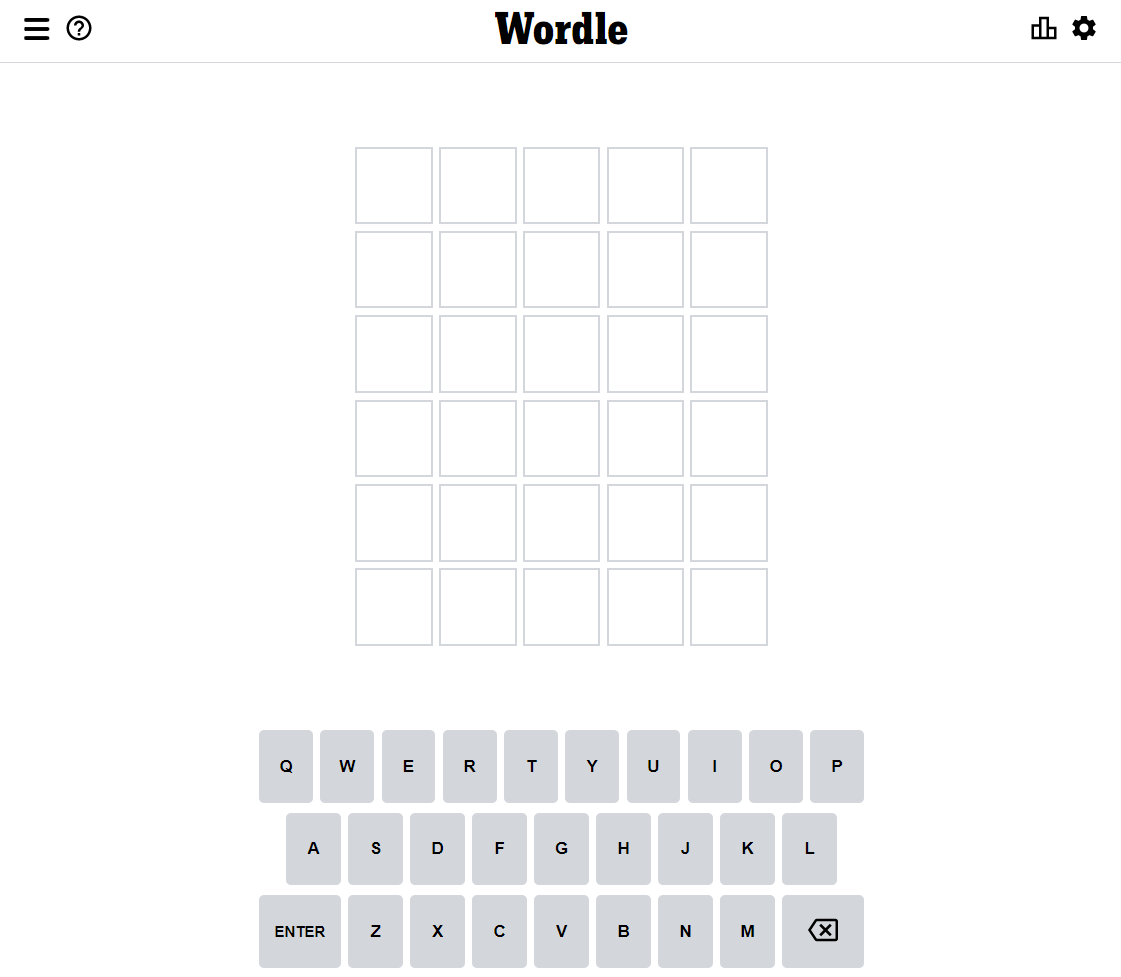
\includegraphics[width=.8\linewidth]{figures/wordle.jpeg}
\end{subfigure}%
\begin{subfigure}{.5\textwidth}
  \centering
  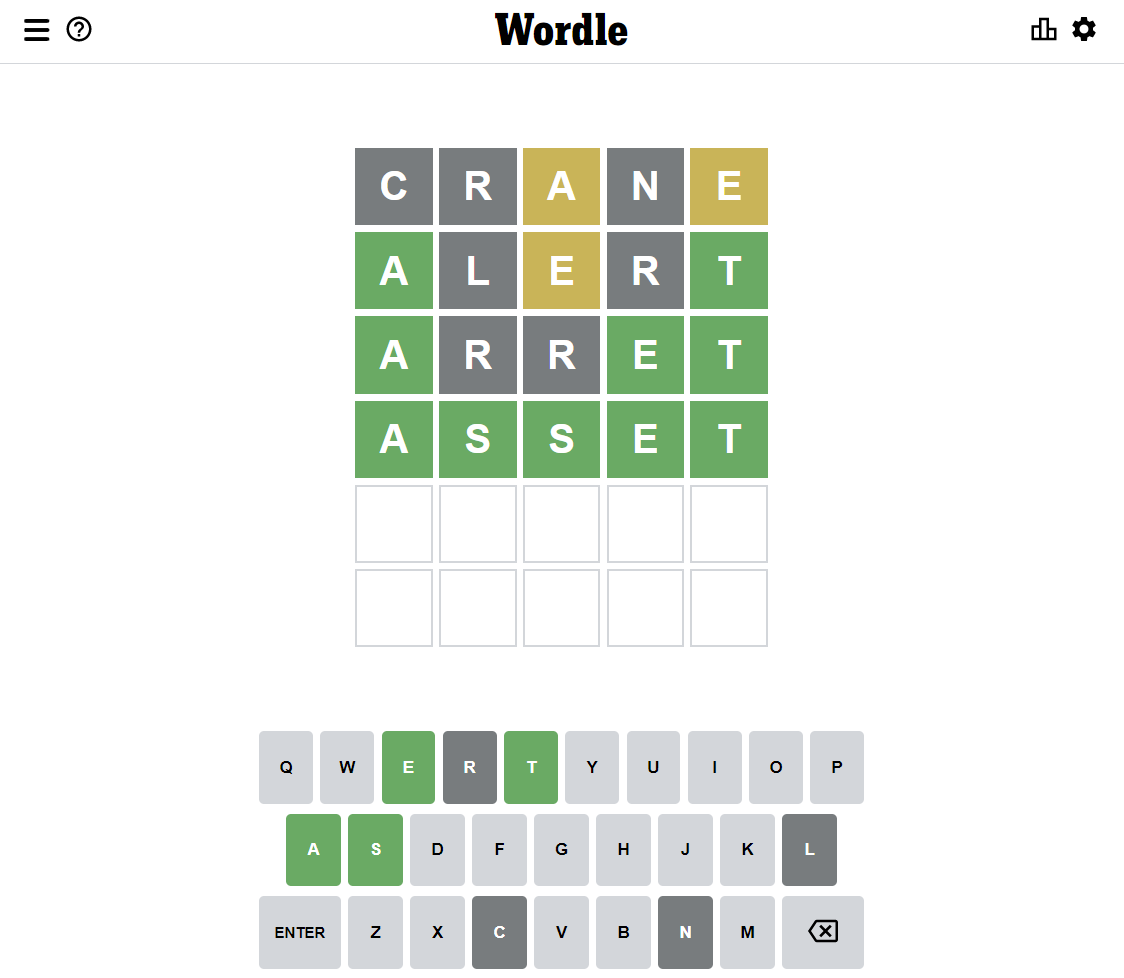
\includegraphics[width=.8\linewidth]{figures/wordle_asset.jpeg}
\end{subfigure}
\caption{Wordle - The New York Times}
\label{fig:test}
\end{figure}

\tabto{1cm}Le joueur a  jusqu'à six tentatives pour deviner un mot de cinq lettres. Après chaque tentative, le jeu montre les lettres qui correspondent à la réponse ; si l'une des 5 lettres devinées apparaît dans la réponse et a également été placée au bon endroit, elle est mise en évidence en vert. Si la lettre apparaît dans la réponse mais n'a pas été placée au bon endroit, elle est sur-lignée en jaune. Si la lettre est complètement fausse, elle devient grise. \\ \\
\tabto{1cm}En bas de la page, le joueur peut voir un clavier QWERTY avec les lettres utilisées sur-lignées en vert, jaune ou gris en fonction des essais précédents. Le joueur peut seulement essayer des mots existants dans le dictionnaire de mots possibles, c'est-à-dire que le joueur ne peut pas rentrer des mots aléatoires ou inexistants dans le but d'obtenir des indices plus rapidement (exemple : AEIOU en français). S’il essaye un mot qui n’est pas dans le dictionnaire, le jeu ne l’accepte pas et le joueur doit en proposer un autre.

\tabto{1cm}

